
\subsection{Machine Readable Zone}

\subsubsection{Construction}
\begin{itemize}
    \item An Machine Readable Zone is composed of two lines of 44 characters
    \item Numbers and punctuations not authorized in the name field
    \item Hyphens are replaced by a filler character ('<')
    \item Apostrophes and commas are omitted
    \item First and last names are separated by 2 filler characters
    \item White characters are replaced by filler characters
\end{itemize}

\subsubsection{Check Digits Calculation}
Check digits are computed for each protecfields. They are calculated modulo 10
with continous repetitive weihting of 731
\begin{itemize}
    \item Letters are mapped to their corresponding numerical value:
    A=10, B=11, \ldots, Z=35, '<'=0.
    \item From left to right, each numerical value is multiplied by the weight
    appearing in the same sequential position.
    \item The product of each multiplication is added modulo 10
\end{itemize}

\paragraph{Example} Calculate the check digit of the document number "EH123456<"

\begin{tabular}{m{10cm}m{6cm}}
    \begin{tabular}{|c|c|c|c|c|c|c|c|c|c|}
        \hline
        Number & E & H & 1 & 2 & 3 & 4 & 5 & 6 & < \\
        & 14 & 17 & 1 & 2 & 3 & 4 & 5 & 6 & 0 \\
        \hline
        Weight & 7 & 3 & 1 & 7 & 3 & 1 & 7 & 3 & 1\\
        \hline
        $N\times W \mod{10}$ & 98 & 51 & 1 & 14 & 9 & 4 & 35 & 18 & 0\\
        \hline
    \end{tabular}
    &
    \begin{eqnarray*}
        98+51+1+14+9+4+35+18 &=& 230 \\
        230 \mod 10 &=& 0 
        \end{eqnarray*}
        $\Rightarrow$ The remainder of the division is the check digit $0$.
\end{tabular}

\subsection{DOC 9303}

\begin{center}
    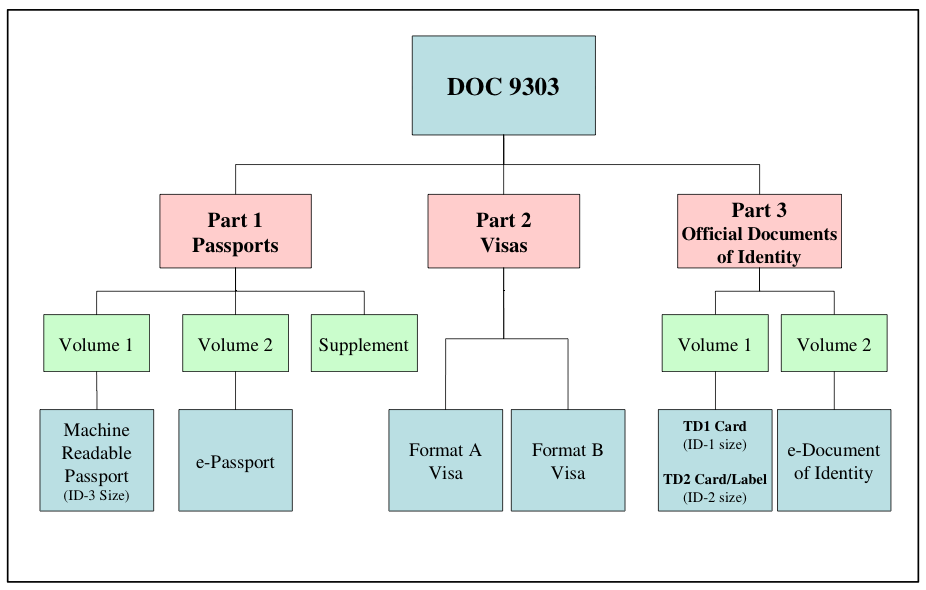
\includegraphics[width=11cm]{img/9303.png}
    \end{center}

\subsubsection{Technical facts about the passport}
\begin{itemize}
    \item Tag is passive (no internal battery)
    \item Tag has a microprocessor (public-key crypto)
    \item Official distance is 10cm
    \item EEPROM capacity: 32KB (minimum)
\end{itemize}

\subsubsection{Passport Content}
\begin{tabular}{|m{2cm}|m{7cm}|m{6cm}|}
    \hline
    Publicly & Publicly possibly after authentication & Never supplied
    by the tag \\
    \hline
    \begin{itemize}
        \item UID 
    \end{itemize}
    &
    \begin{itemize}
        \item Some data groups (DG)
        \item List of data groups on the considered passport (COM)
        \item Cryptographic material signature and hashes (SOD)
    \end{itemize}
    &
    \begin{itemize}
        \item Two symmetric key $K_{ENC},K_{MAC}$ (can be retrieved from MRZ)
        \item One private key $K_{pr}$ (protected memory)
    \end{itemize}
    \\
    \hline
\end{tabular}


\subsection{Protection Mechanisms}
\begin{center}
    \begin{tikzpicture}[node distance= 0.3cm]
        \node [draw=blue, rectangle, text width=5cm] (A) {Modifying data
            of a given passport. Forging a fake passport};

        \node [draw=blue, rectangle, text width=5cm, below=of A] (B) {Cloning a given passport};
        \node [draw=red, rectangle, text width=5cm, below=of B] (C) {Skimming a passport};
        \node [draw=red, rectangle, text width=5cm, below=of C] (D) {Eavesdropping the communication};

        \node [right=2cm of A, text width=4cm] (AA) {Passive Authentication};
        \node [right=2cm of B, text width=4cm] (BB) {Active Authentication};
        \node [right=2cm of C, text width=4cm] (CC) {Basic Access Control};
        \node [right=2cm of D, text width=4cm] (DD) {Secure Messaging};

        \node [right=0cm of AA]  {(Signature)};
        \node [right=0cm of BB]  {(Challenge Response)};
        \node [right=0cm of CC]  {(Reader Authentication)};
        \node [right=0cm of DD]  {(Encryption)};

        \draw[->, >=latex, blue] (AA) to node[] {} (A);
        \draw[->, >=latex, blue] (BB) to node[] {} (B);
        \draw[->, >=latex, red] (CC) to node[] {} (C);
        \draw[->, >=latex, red] (DD) to node[] {} (D);


    \end{tikzpicture}
\end{center}

\subsubsection{Passive Authentication (PA)}
Passive authentication is a \textbf{mandatory security mechanism}: it proves
that the file EF.SOD and LDS are authentic and not modified.

\begin{tabular}{m{8cm}m{7cm}}
    \centering
\begin{tikzpicture}[node distance=0.2cm]
    \node[text width=1.5cm,text centered, rectangle, draw] (1) {$EF.COM$};
    \node[text width=1.5cm,text centered, rectangle, draw, below=of 1] (2) {$DG_1$};
    \node[text width=1.5cm,text centered, rectangle, draw, below=of 2] (3) {$DG_2$};
    \node[text width=1.5cm,text centered,  below=of 3] (4) {$\vdots$};
    \node[text width=1.5cm,text centered, rectangle, draw, below=of 4] (5) {$DG_n$};

    \node[rectangle, draw, dotted, right=0.5cm of 2] (H1) {$hash$};
    \node[rectangle, draw, dotted, right=0.5cm of 3] (H2) {$hash$};
    \node[below=0.5cm of H2] (H3) {$\vdots$};
    \node[rectangle, draw, dotted, right=0.5cm of 5] (H4) {$hash$};

    \node[rectangle, draw,text width=2.5cm, text centered, dotted, right=1cm of H3] (S) {Signature};
    \node[rectangle, draw,text width=2.5cm, text centered, dotted, below =of S] (D) {DS certificate};

    \node[above right=-0.2cm and 1.3cm of H1] (EF) {$EF.SOD$};

    \node [draw, double, rectangle, fit={(H1) (H2) (H3) (H4) (D) (EF) }] (FF) {};

    \node [draw, red, dashed, rectangle, fit={(2) (H1)}] (FF) {};
    \node [draw, red, dashed, rectangle, fit={(3) (H2)}] (FF) {};
    \node [draw, red, dashed, rectangle, fit={(5) (H4)}] (FF) {};
\end{tikzpicture}
& 
\begin{itemize}
    \item \textbf{EF.SOD} contains the hash value of each present
        \textbf{DG}, and signature calculated by the issuing State over values.
    \item The signature can be checked using the Document Signer
        (\textbf{DS}) X.509 certificate. (Available from \textbf{EF.SOD})
    \end{itemize}
\end{tabular}

\begin{itemize}
    \item The DS certificate can be checked using the Country Signing CA (CSCA)
    X.509 cerficate.
    \begin{itemize}
        \item The ICAO PKD does not publish the CSCA certificates
        \item CSCA certificates and revocation lists should be exchanged
        according to bilateral agreements
    \end{itemize}
\end{itemize}

\paragraph{Recommandation} According to DOC 9303:
\begin{itemize}
    \item The passive authentication should use \textsc{RSA},
        \textsc{DSA} or \textsc{ECDSA} for the
    signature schemes
    \item SHA-1, SHA-224/256/384/512 for the hash algorithm
    \item CSCA keys should be renewed every 3-5~years and the DS
    keys every 3~months
\end{itemize}

\subsubsection{Active Authentication (AA)}

The active authentication is an optional security mechanism:
it prove that the \textbf{EF.SOD} belongs to the authentic ePassport, i.e
it is not a cloned one.

\begin{center}
\begin{tabular}{rcl}
    \bf Reader & & \bf ePassport\\
               & \fr{$M_2$} & \\
               & \fl{$Sign(M_2, M_1)$} & \\
    \end{tabular}
\end{center}

\begin{itemize}
    \item Two-pass CR protocol ISO 9796i\text{-}2 Digital Signature Scheme 1
    \item ePassport's public key is stored in DG15
\end{itemize}

The active authentication should rely on RSA, DSA or ECDSA with minimum sizes for
the security parameters should be respectively 1024 bits, 1024 and 160
bits, and 160 bits.

\paragraph{Example with RSA/SHA~1}

\begin{center}
\begin{tabular}{rcl}
    \bf Reader & & \bf ePassport\\
    $M_2 \in_R \{0, 1\}^{64}$   & \fr{$M_2$} & $M_1 \in_R \{0, 1\}^{848}$ \\
                                & & $F = 6A||M_1||SHA1(M_1, M_2)||BC$\\
    $F^* = RSA_{PK_{DG15}}(S)$ &\fl{$S$} & $S = RSA_{SK_{DG15}}(F)$ \\
    $6A||M_1^*||H^*||T^* = F^*$ & & \\
    $SHA1(M_1^*||M_2) ?=? H^*$ &&\\
    \end{tabular}
\end{center}

\subsubsection{Basic Access Control (BAC) and Secure Messaging (SM)}

\begin{tikzpicture}
    \footnotesize
    \node (BAC) {\bf Basic Access Control};
\node[below=0cm of BAC, text width=3.3cm] (BAC1) {\begin{tabular}{l}Encryption Key\\ MAC Key\end{tabular}};

        \node[below=2cm of BAC] (SM) {\bf Secure Messaging};
    \node[below=0cm of SM, text width=3.3cm] (SM1) {\begin{tabular}{l}Session Encryption
    Key\\ Session MAC Key\end{tabular}};

    \node[draw, rectangle, above left=0.0cm and 1.5cm of BAC] (MRZ) {\begin{tabular}{l} Passport
        Number\\Expiration Date \\ Birth Date\end{tabular}};
    \node[above=0cm of MRZ] {\bf MRZ};

    \node[draw, rectangle, double, fit={(BAC) (BAC1)}] (BBAC)  {};
    \node[draw, rectangle, double, fit={(SM) (SM1)}] (SSM)  {};

    \draw[->] (MRZ) -| (BBAC);
    \draw[->] (BBAC) -| (-2.5cm, -1.5cm) |- (SSM);

    \node[above left=0.2cm and 1cm of SM] {$K_r, K_p$};

    \node[right=of BBAC] {\scriptsize \begin{tabular}{rcl}
            \bf Reader &&\bf Passport\\
                       &\fl{$C_p$}&\\
                       &\fr{$a = ENC\big(C_p, C_r, K_r\big), MAC(a)$}&\\
                       &\fl{$b = ENC\big(C_p, C_r, K_p\big), MAC(b)$}&\\
            \end{tabular} };

    \node[right=of SSM] {\scriptsize \begin{tabular}{rcl}
            \bf Reader &&\bf Passport\\
                       &\fr{Authenticated Query}&\\
                       &\fr{Encrypted Data}&\\
            \end{tabular} };
\end{tikzpicture}

\begin{itemize}
    \item Three-pass CR protocol according to ISO 11770\text{-}2 Key Establishment
    Mechanism 6, 2-key 3DES as block cipher
    \item Nonces should be 8-byte long
    \item Encryption done using 3DES in CBC mode with zero-IV according to
    ISO 11568\text{-}2
    \item A cryptographic checksum is calculated over: ISO 9797\text{-}1 MAC
    Algorithm 3 (i.e Retail-MAC), based on DES, zero-IV, ISO 9797\text{-}1 Padding
    Method 2
    \item Encryption and MAC keys derived from the MRZ using SHA-1
\end{itemize}

\begin{tabular}{m{3cm}m{11cm}}
\textbf{Key Derivation} &
\begin{enumerate}
    \item Set $ K_{seed} = trunc_{16}(SHA-1(MRZ\_info))\quad or\ (K_r \oplus K_p)$
    \item Set $ D = K_{seed}||00000001 $
    \item Compute $ H = SHA-1(D) $
    \item First 16 bytes of H are set to the 2-key 3DES $ K_{ENC} $
    \item Set $ D = K_{seed}||00000002 $
    \item Compute $ H = SHA-1(D) $
    \item First 16 bytes of H are set to the 2 DES keys $K_{MAC} $
    \item Adjust the parity bits of the DES keys
\end{enumerate}
\end{tabular}

\subsection{Weaknesses}
BAC keys are derived from the MRZ, especially date of birth, date of expiry,
passport number. 

$\Rightarrow$ But passport numbers are usually not random, DOB and DOE are
neither random.

\begin{itemize}
    \item Relay Attacks: Passport is based on ISO 14443, so it can require to
    increase the timeouts.
    \item Evidence of Presence: Abuse the active authentication which can be
    doable without passing the BAC
    \item Chain of Trust: If the root certificate cannot be verified, making a
    fake passport is quite easy
\end{itemize}

\subsubsection{Information leakage through side channel}
An adversary can guess the issuing state of an ePassport without
knowledge of the BAC keys:
\begin{enumerate}
    \item Send wrong messages to the passport
    \item Analyze the error messages.
    \item  Fingerprint the countries.
\end{enumerate}
Error messages are the external signal of an internal behavior.
Implementer have too frequently to deal themselves with the
error messages but they are not aware of potential security issues.

\subsection{Extended Access Control (EAC)}
EAC is an improved security mechanism that aims to eventually
replace BAC and AA.

\begin{itemize}
    \item Includes the tag authentication (should eventually replace AA)
        and the terminal authentication (makes obsolete BAC because
        only authorized readers have access to the data).
\end{itemize}

